\section*{Tests and metrics}

\subsection*{Classic Na\"ive Bayes vs Embeddings}

In figure \ref{fig:classic_nb_vs_embeddings} are shown the ROC curves obtained with the models without preprocessing, the dataset split is set to 80\% for the train set and 20\% for the test one.
We can see how simpler approaches eventually bring the best results, in fact using word embeddings the final score was much lower than the one obtained with the classic na\"ive Bayes with bag of words. From these tests it looks like na\"ive Bayes can't exploit the properties of word embeddings at their best. It is also interesting to note how using the Gaussian model with embeddings turned out to be the worst model, as the values in the embeddings are probably not gaussian.
%Both the simple Bernoulli and the multinomial Na\"ive Bayes that counts words occurrences have reached the maximum accuracy with very similar results.

\begin{figure}[h!t]
    \centering
    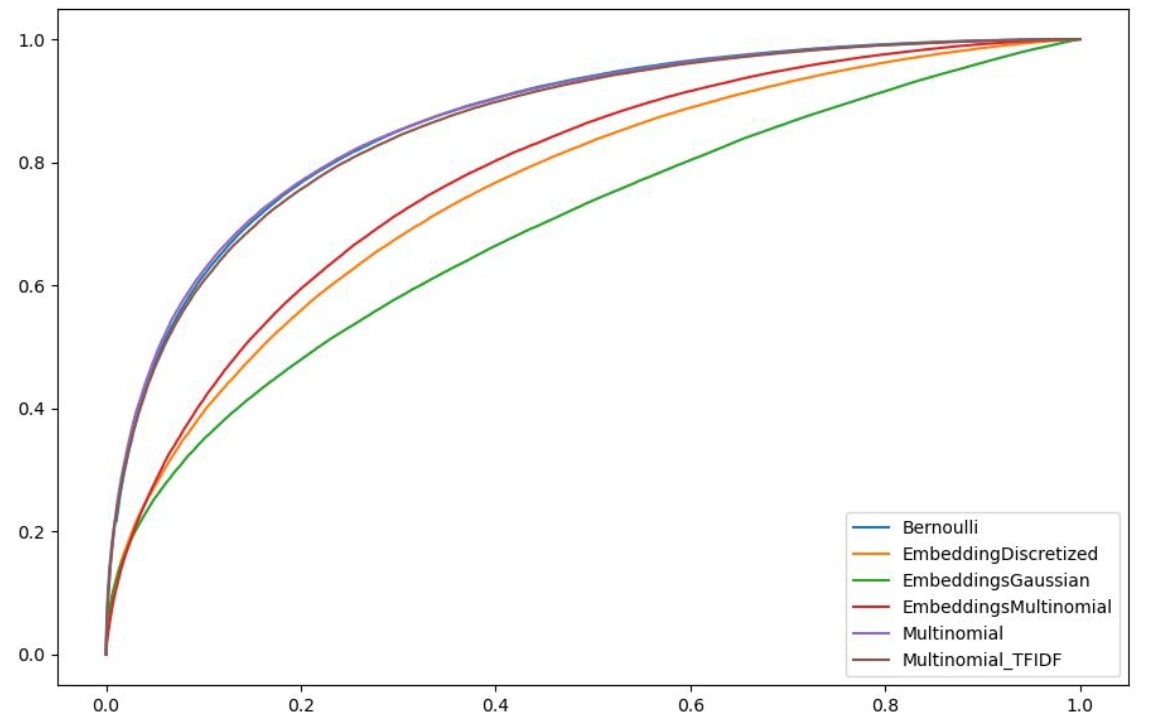
\includegraphics[scale=0.50]{../experiments/plots/classic_nb_vs_embeddings}
    \caption{ROC curves that compare the classic Na\"ive Bayes models and
    word embedding approaches.}
    \label{fig:classic_nb_vs_embeddings}        
\end{figure}

Classical na\"ive Bayes are the best performing models so, focusing on them, some hyperparameter tuning has been applied. The intention has been to find the best n-grams to maximize the final results. In order to do that, 20\% of the dataset has been dedicated to the cross validation set (60\% to training, 20\% to test).
In table \ref{tab:classic_nb_vs_embeddings} we can see some metrics. 
All of their performances are very similar with around 80\% of Accuracy and F1-score and 88\% of AUROC. The best n-grams turned out to be (1-3)-grams (for Bernoulli and Multinomial with tf-idf) and (1-2)-grams for standard multinomial event model.

\begin{table}[h!t]
    \centering
    \caption{Results obtained with bag of words Bernoulli and Multinomial models.}
    \label{tab:classic_nb_vs_embeddings}
    \begin{tabular}{c|ccc}
        \hline
        Model & Accuracy & F1 & AUROC \\
        \hline 
        Bernoulli & 0.797 & 0.799 & 0.880 \\ 
        Multinomial & 0.802 & 0.802 & 0.884 \\ 
        Multinomial TF-IDF & 0.805 & 0.804 & 0.886 \\ 
        \hline
    \end{tabular}
\end{table}

\subsection*{Kaggle notebooks}

In this section we describe how we compared our models to a couple of top-rated notebooks on Kaggle.
We also tried to run these notebooks without removing stopwords from their datasets hoping to gain some further insight on their role in the learning process. 

The model we chose to compare to these notebooks is our best performing one: multinomial na\"ive Bayes with tf-idf. 
The first selected notebook is the best one that uses this same technique ~\cite{startups:notebook1}, we resized our dataset split to match theirs and have a comparison as equal as possible.
We were happy to see that their AUROC score was slightly lower than ours, as showed in \ref{tab:versus_metrics_NB}.
However their performance fairly improved when no processing was applied.

\begin{table}[h!t]
    \centering
    \caption{Model comparision with and without preprocessing.}
    \label{tab:versus_metrics_NB}
    \begin{tabular}{c|c}
        \hline
        Model & AUROC \\
        \hline 
        Notebook & 0.839 \\ 
        Us & 0.841 \\ 
        Notebook no preprocessing & 0.849 \\ 
        \hline
    \end{tabular}
\end{table}

We also wanted to see if more complex models could capture the irregularities in word embeddings better than ours na\"ive Bayes. 
We looked for Kaggle notebooks with best results on word embeddings and found ~\cite{startups:notebook2} who is based on a LSTM neural network.
We were truly surprised to see that its accuracy was lower than the one reached by our tf-idf model, scores are showed in table \ref{tab:versus_metrics_FT}. 
Anyway when emptying the lists of stopwords to be removed from the dataset and running the notebook again its accuracy enjoys a significant boost. 
These results make us support the intuition that some stopwords contain useful information that we want to keep in our dataset. We compared the models using the metric chosen by the authors of the notebooks (AUROC for the first notebook, accuracy for the second one).

\begin{table}[h!t]
    \centering
    \caption{Model comparision with and without stopword removal.}
    \label{tab:versus_metrics_FT}
    \begin{tabular}{c|c}
        \hline
        Model & Accuracy\\
        \hline 
        Notebook & 0.779 \\ 
        Us & 0.799 \\ 
        Notebook with stop-word & 0.816 \\ 
        \hline
    \end{tabular}
\end{table}

\subsection*{Further tests}
We performed some unusual tests: we trained our model with a dataset and tested it against a different one. The motivation behind this test is the following: suppose we have a model which is good in sentiment analysis on tweets, and we would like to do sentiment analisys also on another social network but for which we don't have any data to train on (if we had even a small amount of data, we could try some transfer learning technique), then it is interesting to see if our model trained on twitter can give decent results also on the other social network, or if the results will be basically random.\\
We used an IMDb dataset of cinematographic reviews ~\cite{data:imdb} and a Reddit one about various NFL games\footnote{In this dataset the label is a real value in [-1,1], we considered only the comments with absolute value greater than 0.5, and set their label either to 0 or 1} ~\cite{data:reddit}, results for the Multivariate Bernoulli event model Na\"ive Bayes (using (1,3)-gram\footnote{In a (1-3)-gram we consider 1,2 and 3-grams}) without preprocessing can be seen in figures \ref{fig:TwitterImdb} and \ref{fig:TwitterReddit}.

\begin{figure}[h!t]
    \centering
    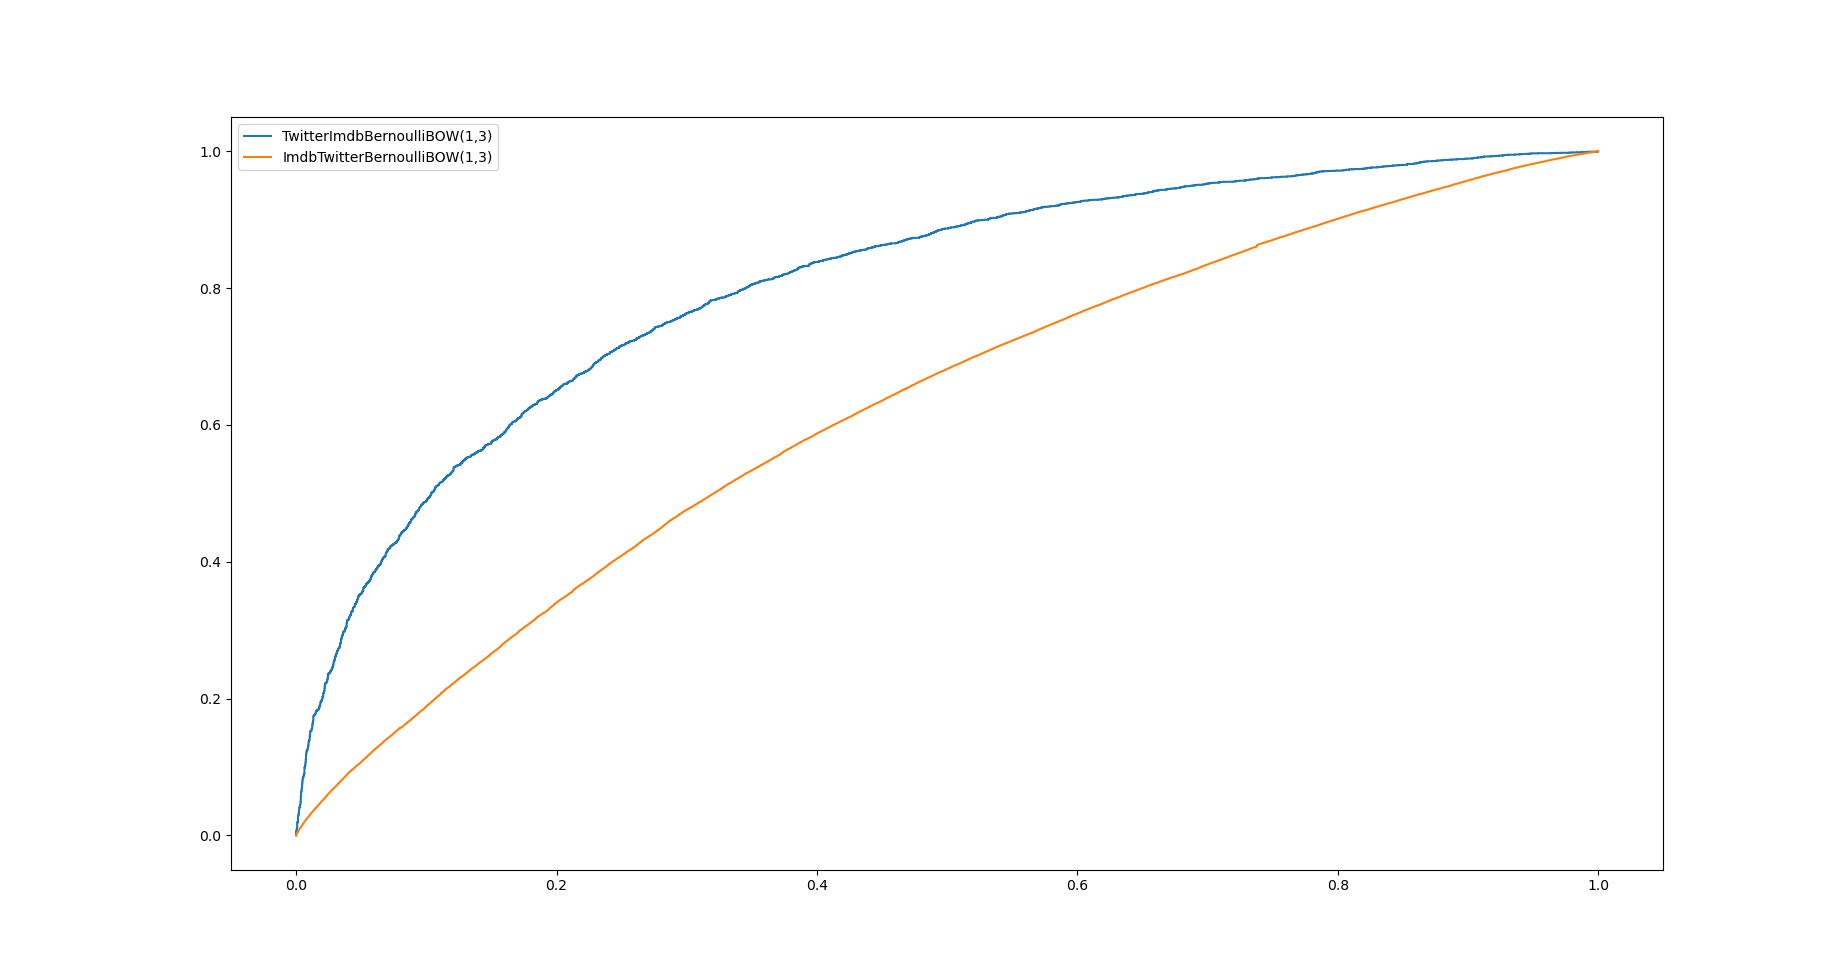
\includegraphics[scale=0.3]{../experiments/plots/ImdbTwitter}
    \caption{Comparison between Imdb-Twitter (training on Imdb, testing on Twitter) and Twitter-Imdb (training on Twitter, testing on Imdb).}
    \label{fig:TwitterImdb}        
\end{figure}

\begin{figure}[h!t]
    \centering
    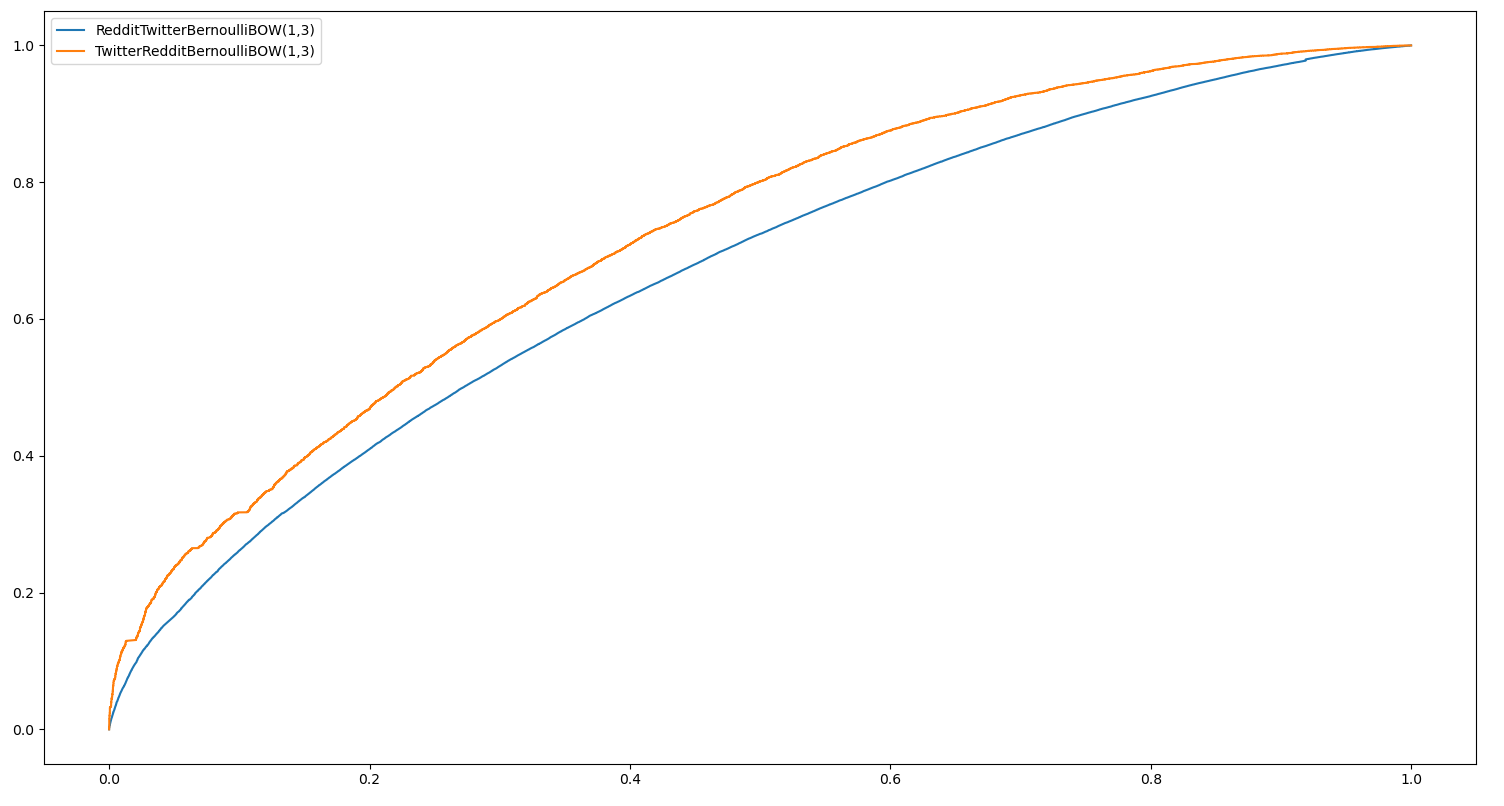
\includegraphics[scale=0.3]{../experiments/plots/RedditTwitter}
    \caption{Comparison betwen Reddit-Twitter (training on Reddit, testing on Twitter), and Twitter-Reddit (training on Twitter, testing on Reddit).}
    \label{fig:TwitterReddit}
\end{figure}

This is something usually not done since different datasets will have different distributions hence we expect bad results and this is what we got except for one particular case.
Training our model with the Twitter dataset and testing it with the IMDb one strangely gives us rather good metrics, this can be seen in table \ref{tab:versus_metrics} where only the comparision betwen Twitter and IMDb is shown since results are more interesting. 

This could be due to Twitter's dataset being very large while other datasets are smaller and also very specific.
The Reddit one is only about a specific set of american football games and the IMDb one is about cinematographic reviews, reasonably in this case lexicon is also more specific than arbitrairly picked tweets.
On the other hand Sentiment140 covers a wider class of human language and is less prone to be biased.


\begin{table}[h!t]
    \centering
    \caption{Comparing metrics for some train test combinations (using Bernoulli event model). Twitter-IMDb is surprisingly not bad (even though still worse than training and testing directly on IMDb)}
    \label{tab:versus_metrics}
    \begin{tabular}{c|ccc}
        \hline
        Train-Test & Accuracy & F1 & AUROC \\
        \hline 
        Twitter-IMDb & 0.732 & 0.723 & 0.806 \\ 
        IMDb-IMDb & 0.891 & 0.887 & 0.963 \\ 
        IMDb-Twitter & 0.550 & 0.330 & 0.625 \\ 
        Twitter-Twitter & 0.797 & 0.799 & 0.880 \\ 
        \hline
    \end{tabular}
\end{table}
